% !TeX program = lualatex
\documentclass{beamer}

\usepackage{csquotes}
%\usepackage{enumerate}
\usepackage{mathtools}
\usepackage{unicode-math}
\usepackage{tensor}
\usepackage{diffcoeff}

\usepackage{ytableau}
\ytableausetup{centertableaux}

\usepackage{tikz}
\usetikzlibrary{positioning, calc}
\colorlet{background color}{black!2}
\tikzset{wire/.style={thick}}
\tikzset{underwire/.style={line width=1mm, background color}}
\tikzset{symmetriser/.style={fill=background color, thick, rounded corners=1pt}}
\tikzset{antisymmetriser/.style={fill, thick, rounded corners=1pt}}


\title{Computational Group Theory}
\subtitle{MPhys Project Presentation}
\author{Willoughby Seago\texorpdfstring{\\}{} Supervised by Anthony Kennedy}
\institute{The University of Edinburgh}
\date{}

\usetheme[progressbar=frametitle]{metropolis}
\setbeamertemplate{frame numbering}[fraction]
\useoutertheme{metropolis}
\useinnertheme{metropolis}
\usefonttheme{metropolis}
\definecolor{edinburghblue}{HTML}{041E42}
\definecolor{edinburghred}{HTML}{D50032}
\usecolortheme[named=edinburghblue]{structure}
\setbeamercolor{alerted text}{fg=edinburghred,bg=edinburghblue}

\metroset{block=fill}

\newcommand{\define}[1]{\alert{#1}}
\newcommand{\vv}[1]{\symbf{#1}}
\DeclarePairedDelimiter{\abs}{\lvert}{\rvert}
\newcommand{\ve}[1]{\vv{e}_{#1}}
\newcommand{\complex}{\symbb{C}}
\newcommand{\reals}{\symbb{R}}
\newcommand{\quaternions}{\symbb{H}}
\newcommand{\groupAction}{\mathbin{.}}
\newcommand{\grad}{\nabla}
\newcommand{\curl}{\nabla\times}
\DeclareMathOperator{\specialUnitary}{SU}
\DeclareMathOperator{\unitary}{U}
\DeclareMathOperator{\specialOrthogonal}{SO}
\DeclareMathOperator{\symplectic}{Sp}

\begin{document}
    
    \begin{frame}
        \vspace{2ex}
        \includegraphics[width=0.6\textwidth]{sopa-logo}\\
        \vspace*{-1.93cm}
        \titlepage
    \end{frame}
    
    \begin{frame}
        \tableofcontents
    \end{frame}
    
    \section{Tensor Symmetry}
    \begin{frame}{Overview}
        Tensors appear everywhere in physics.
        
        Often they have some symmetry we can exploit to simplify calculations.
        
        This is what my project is on:
        \begin{itemize}
            \item\pause understanding the maths behind this, which comes from the fields of group theory and representation theory
            \item\pause writing code to simplify tensor expressions exploiting these symmetries using this maths
        \end{itemize}
        \pause
        This presentation will give an overview of the theory.
    \end{frame}

    \begin{frame}{Kronecker Delta}
        Kronecker delta:
        \begin{equation*}
            \delta^{ij} = 
            \begin{cases}
                1 & i = j,\\
                0 & i \ne j.
            \end{cases}
        \end{equation*}
        This is \define{totally symmetric}:
        \begin{equation*}
            \delta^{ij} = \delta^{ji}.
        \end{equation*}
    \end{frame}
    
    \begin{frame}{Field Strength Tensor}
        Combine \(\vv{E}\) and \(\vv{B}\) fields into one tensor:
        \begin{equation}
            F^{\mu\nu} =
            \begin{pmatrix}
                0 & -E_x & -E_y & -E_z\\
                E_x & 0 & -B_z & B_y\\
                E_y & B_z & 0 & -B_x\\
                E_z & -B_y & B_x & 0
            \end{pmatrix}
            .
            \tag{\(c = 1\)}
        \end{equation}
        This is \define{totally antisymmetric}:
        \begin{equation*}
            F^{\mu\nu} = -F^{\nu\mu}.
        \end{equation*}
    \end{frame}
    
    \begin{frame}{Levi--Civita Symbol}
        Levi--Civita:
        \begin{equation*}
            \varepsilon^{ijk} =
            \begin{cases}
                1 & ijk \in \{123, 231, 312\},\\
                -1 & ijk \in \{132, 213, 321\},\\
                0 & \text{otherwise}.
            \end{cases}
        \end{equation*}
        This is \define{totally antisymmetric}:
        \begin{equation*}
            \varepsilon^{ijk} = -\varepsilon^{jik} = -\varepsilon^{ikj} = -\varepsilon^{kji}.
        \end{equation*}
    \end{frame}
    
    \begin{frame}{Riemann Tensor}
        The Riemann tensor, \(R_{\mu\nu\rho\sigma}\), measures curvature in general relativity.
        
        \pause
        The Riemann tensor has the following symmetries:
        \begin{align*}
            R_{\mu\nu\rho\sigma} &= - R_{\nu\mu\rho\sigma},\\
            R_{\mu\nu\rho\sigma} &= - R_{\mu\nu\sigma\rho},\\
            R_{\mu\nu\rho\sigma} &= \hphantom{-} R_{\rho\sigma\mu\nu}.
        \end{align*}
        
        This is clearly quite a bit more complicated than our other examples.
    \end{frame}
    
    \section{Classifying Symmetries}
    
    \begin{frame}{Exploiting Symmetry}
        We've seen a variety of symmetries:
        \begin{itemize}
            \item Totally symmetric: \(\delta^{ij}\)
            \item Totally antisymmetric: \(F^{\mu\nu}\), \(\varepsilon^{ijk}\)
            \item A mixture: \(R_{\mu\nu\rho\sigma}\)
        \end{itemize}
        \pause
        Exploiting these symmetries efficiently can greatly simplify calculations, e.g.
        \begin{align*}
            \delta^{ij}\varepsilon^{ijk} &= 0\\
            F^{\mu\nu}F_{\mu\nu} &= 2(\partial^\mu A^\nu)F_{\mu\nu}, \qquad \text{(1/2 as many terms)}\\
            R_{\mu\nu\rho\sigma} + R_{\mu\rho\sigma\nu} + R_{\mu\sigma\nu\rho} &= 0.
        \end{align*}
    \end{frame}
    
    \begin{frame}{The Symmetric Group}
        To exploit these symmetries we need to classify them.
        This can be done using the \define{symmetric group}.
        
        \pause
        \begin{definition}
            The \define{symmetric group}, \(S_n\), is the set of all permutations of \(n\) objects.
            Two permutations are combined by performing them one after another.
            We think of this as multiplying the two permutations.
        \end{definition}
    \end{frame}
    
    \begin{frame}{Classifying Tensor Symmetries}
        Classify tensor symmetries using \define{Young Tableaux}.
        
        Diagrams made from numbered boxes, which tell us about the symmetry of an object.
        
        \pause
        Put symmetric pairs of indices in the same row
        
        Represent the symmetry of \(\delta^{ij}\) with
        \begin{equation*}
            \ytableaushort{ij}.
        \end{equation*}
        
        \pause
        Put antisymmetric pairs of indices in the same column
        
        Represent the antisymmetry of \(F^{\mu\nu}\) and \(\varepsilon^{ijk}\) as
        \begin{equation*}
            \ytableaushort{\mu,\nu}, \qquad\text{and}\qquad \ytableaushort{i,j,k}.
        \end{equation*}
    \end{frame}
    
    \begin{frame}{Classifying Symmetries of the Riemann Tensor}
        The Riemann tensor has more complicated symmetries.
        \begin{itemize}
            \item \(R_{\mu\nu\rho\sigma} = -R_{\nu\mu\rho\sigma}\) tells us \(\mu\) and \(\nu\) are in the same column.
            \item \(R_{\mu\nu\rho\sigma} = -R_{\mu\nu\sigma\rho}\) tells us \(\rho\) and \(\sigma\) are in the same column.
            \item \(R_{\mu\nu\rho\sigma} = R_{\rho\sigma\mu\nu}\) tells us that \(\mu\) and \(\rho\), as well as \(\nu\) and \(\sigma\), must be on the same row.
        \end{itemize}
        \pause
        Hence, the symmetries of \(R_{\mu\nu\rho\sigma}\) are represented by
        \begin{equation*}
            \ytableaushort{\mu\rho,\nu\sigma}.
        \end{equation*}
    \end{frame}
    
    \section{Young Projectors}
    \begin{frame}{Symmetrisers}
        Tensor without symmetry \(\to\) tensor with symmetry
        
        Take linear combinations of permutations.
        
        \pause
        Totally symmetric \(\to\) symmetrise \(\to\) sum over permutations:
        \begin{equation*}
            T^{(\mu\nu)} = S_{12} \groupAction T^{\mu\nu} = \frac{1}{2!}(T^{\mu\nu} + T^{\nu\mu}).
        \end{equation*}
        \pause
        Totally antisymmetric \(\to\) antisymmetrise \(\to\) alternating sum over permutations:
        \begin{equation*}
            T^{[\mu\nu]} = A_{12} \groupAction T^{\mu\nu} = \frac{1}{2!}(T^{\mu\nu} - T^{\nu\mu}).
        \end{equation*}
    \end{frame}
    
    \begin{frame}{Diagrammatic Notation}
        We can represent a permutation as a diagram with wires tracking the elements through the permutation, for example
        \begin{equation*}
            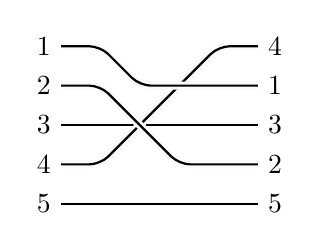
\begin{tikzpicture}[baseline=(current bounding box)]
                \draw[wire] (0, 0.5) node [left] {5} -- (2.5, 0.5) node [right] {5};
                \draw[wire] (0, 1.5) node [left] {3} -- (2.5, 1.5) node [right] {3};
                \draw[underwire, rounded corners] (0, 1) -- (0.5, 1) -- (2, 2.5) -- (2.5, 2.5);
                \draw[wire, rounded corners] (0, 1) node [left] {4} -- (0.5, 1) -- (2, 2.5) -- (2.5, 2.5) node [right] {4};
                \draw[underwire, rounded corners] (0, 2.5) -- (0.5, 2.5) -- (1, 2) -- (2.5, 2);
                \draw[wire, rounded corners] (0, 2.5) node [left] {1} -- (0.5, 2.5) -- (1, 2) -- (2.5, 2) node [right] {1};
                \draw[underwire, rounded corners] (0, 2) -- (0.5, 2) -- (1.5, 1) -- (2.5, 1);
                \draw[wire, rounded corners] (0, 2) node [left] {2} -- (0.5, 2) -- (1.5, 1) -- (2.5, 1) node [right] {2};
            \end{tikzpicture}
        \end{equation*}
        represents the permutation
        \begin{equation*}
            1 \to 2, \quad 2 \to 4, \quad 3 \to 3, \quad 4 \to 1, \quad 5 \to 5
        \end{equation*}
        or \((1\, 2\, 4)\) in cycle notation, where each element is sent to the next one in the list, and the list wraps round to the start at the end.
    \end{frame}
    
    \begin{frame}{Symmetriser}
        In this notation symmetrising over indices is written with an empty box:
        \begin{equation*}
            S_{12} = 
            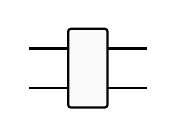
\begin{tikzpicture}[baseline=0.15cm]
                \draw[wire] (-0.5, 0) -- (0, 0);
                \draw[wire] (-0.5, 0.5) -- (0, 0.5);
                \draw[symmetriser] (0, -0.25) rectangle (0.5, 0.75);
                \draw[wire] (0.5, 0) -- (1, 0);
                \draw[wire] (0.5, 0.5) -- (1, 0.5);
            \end{tikzpicture}
            = \frac{1}{2} \Big[\,
            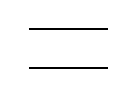
\begin{tikzpicture}[baseline=0.15cm]
                \draw[wire] (0, 0) -- (1, 0);
                \draw[wire] (0, 0.5) -- (1, 0.5);
            \end{tikzpicture}
            +
            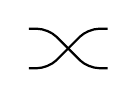
\begin{tikzpicture}[baseline=0.15cm]
                \draw[wire, rounded corners] (0, 0) -- (0.25, 0) -- (0.75, 0.5) -- (1, 0.5);
                \draw[wire, rounded corners] (0, 0.5) -- (0.25, 0.5) -- (0.75, 0) -- (1, 0);
            \end{tikzpicture}
            \,\Big]
            = \frac{1}{2}[() + (1\, 2)]
        \end{equation*}
        \pause
        Similarly, antisymmetrisation is represented by a filled box:
        \begin{equation*}
            A_{12} = 
            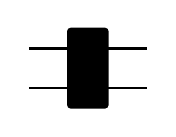
\begin{tikzpicture}[baseline=0.15cm]
                \draw[wire] (-0.5, 0) -- (0, 0);
                \draw[wire] (-0.5, 0.5) -- (0, 0.5);
                \draw[antisymmetriser] (0, -0.25) rectangle (0.5, 0.75);
                \draw[wire] (0.5, 0) -- (1, 0);
                \draw[wire] (0.5, 0.5) -- (1, 0.5);
            \end{tikzpicture}
            = \frac{1}{2} \Big[\,
            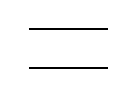
\begin{tikzpicture}[baseline=0.15cm]
                \draw[wire] (0, 0) -- (1, 0);
                \draw[wire] (0, 0.5) -- (1, 0.5);
            \end{tikzpicture}
            -
            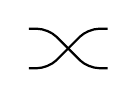
\begin{tikzpicture}[baseline=0.15cm]
                \draw[wire, rounded corners] (0, 0) -- (0.25, 0) -- (0.75, 0.5) -- (1, 0.5);
                \draw[wire, rounded corners] (0, 0.5) -- (0.25, 0.5) -- (0.75, 0) -- (1, 0);
            \end{tikzpicture}
            \,\Big]
            = \frac{1}{2}[() - (1\, 2)]
        \end{equation*}
    \end{frame}
    
    \begin{frame}{Young Projectors}
        We can generate tensors with any symmetry using Young projectors, which we get from Young tableaux:
        \begin{itemize}
            \item Symmetrise over rows
            \item Antisymmetrise over columns
        \end{itemize}
        For example:
        \begin{equation*}
            \ytableaushort{12,34} \propto
            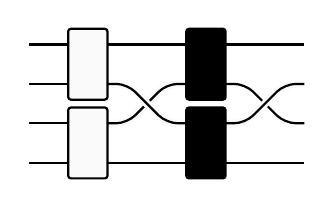
\begin{tikzpicture}[baseline=0.65cm, font=\small]
                \foreach \y in {0, 0.5, 1, 1.5} {
                    \draw[wire] (-0.5, \y) -- (0, \y);
                }
                
                \draw[wire] (0.5, 1.5) -- (1.5, 1.5);
                \draw[wire] (0.5, 0) -- (1.5, 0);
                \draw[rounded corners, underwire] (0.5, 0.5) -- (0.75, 0.5) -- (1.25, 1) -- (1.5, 1);
                \draw[wire, rounded corners] (0.5, 0.5) -- (0.75, 0.5) -- (1.25, 1) -- (1.5, 1);
                \draw[rounded corners, underwire] (0.5, 1) -- (0.75, 1) -- (1.25, 0.5) -- (1.5, 0.5);
                \draw[wire, rounded corners] (0.5, 1) -- (0.75, 1) -- (1.25, 0.5) -- (1.5, 0.5);
                
                \draw[wire] (2, 0) -- (3, 0);
                \draw[wire] (2, 1.5) -- (3, 1.5);
                \draw[wire, rounded corners] (2, 1) -- (2.25, 1) -- (2.75, 0.5) -- (3, 0.5);
                \draw[underwire, rounded corners] (2, 0.5) -- (2.25, 0.5) -- (2.75, 1) -- (3, 1);
                \draw[wire, rounded corners] (2, 0.5) -- (2.25, 0.5) -- (2.75, 1) -- (3, 1);
                
                \draw[symmetriser] (0, -0.2) rectangle (0.5, 0.7);
                \draw[symmetriser] (0, 0.8) rectangle (0.5, 1.7);
                \draw[antisymmetriser] (1.5, -0.2) rectangle (2, 0.7);
                \draw[antisymmetriser] (1.5, 0.8) rectangle (2, 1.7);
            \end{tikzpicture}
        \end{equation*}
        Expanding the (anti)symmetrisers we have \(2^4 = 16\) terms, these get out of hand quickly.
    \end{frame}
    
    \begin{frame}{Representation}
        The permutations in the symmetric group can act on tensors, and this is done through a \define{representation}, a collection of matrices
        \begin{equation*}
            \{\rho(\sigma) \mid \sigma \in S_n\}
        \end{equation*}
        with the same multiplication rules as the symmetric group, so
        \begin{equation*}
            \underbrace{\rho(\sigma)\rho(\tau)}_{\parbox{3cm}{\scriptsize product of two matrices, \(\rho(\sigma)\) and \(\rho(\tau)\)}} = \hspace{1cm} \rho(\underbrace{\sigma\tau}_{\mathclap{\parbox{3cm}{\scriptsize product of two permutations, \(\sigma\) and \(\tau\)}}})
        \end{equation*}
        These are much easier to work with, but, we have to find them first.
        This is what most of my code has focused on so far.
    \end{frame}
    
    
    \begin{frame}{What Else?}
        \begin{itemize}
            \item\pause Expanding (anti)symmetrisers \(\symcal{O}(2^n)\) \(\to\) Use Garnir relations to efficiently calculate representations (Done)
            \item\pause Computing \(3j\) and \(6j\) coefficients (In progress)
            \item\pause Hermitian Young projectors (In progress)
            \item\pause Other groups (Future work)
            \begin{itemize}
                \item\pause Currently \(\specialUnitary(N)\), good for spin (\(\specialUnitary(2)\)), QCD (\(\specialUnitary(3)\)), Yang--Mills (\(\specialUnitary(N)\)), electroweak (\(\specialUnitary(2)_{\symrm{L}} \times \unitary(1)_{Y}\)).
                \item\pause \(\specialOrthogonal(n)\) \(\to\) Rotations \(\to\) Classical Mechanics
                \item\pause \(\specialOrthogonal(1, 3)\) \(\to\) Lorentz transformations \(\to\) Relativity
                \item\pause \(\symplectic(2n)\) \(\to\) Transformations preserving Hamilton's equations \(\to\) Hamiltonian Dynamics
            \end{itemize}
        \end{itemize}
    \end{frame}
    
    \section{Any Questions?}
    
    \begin{frame}{What's the Field Strength Tensor?}
        Suppose we have a scalar potential, \(\varphi\), and vector potential \(\vv{A}\).
        
        The electric and magnetic fields are then
        \begin{equation*}
            \vv{E} = -\grad \varphi - \diffp{\vv{A}}{t}, \quad\text{and}\quad \vv{B} = \curl \vv{A}.
        \end{equation*}
        
        We can define the four-potential, \(A^\mu = (\varphi, \vv{A})\) (\(c = 1\)), then we have
        \begin{equation*}
            F^{\mu\nu} = \partial^\mu A^\nu - \partial^\nu A^\mu =
            \begin{pmatrix}
                0 & -E_x & -E_y & -E_z\\
                E_x & 0 & -B_z & B_y\\
                E_y & B_z & 0 & -B_x\\
                E_z & -B_y & B_x & 0
            \end{pmatrix}
            \tag{\(c = 1\)}
        \end{equation*}
    \end{frame}
    
    \begin{frame}{What's the Riemann Tensor?}
        One way of defining the Riemann tensor is as follows:
        \begin{equation*}
            \tensor{R}{^\mu_{\nu\rho\sigma}} = \partial_\rho \tensor{\Gamma}{^\mu_{\nu\sigma}} - \partial_\sigma \tensor{\Gamma}{^\mu_{\rho\nu}} + \tensor{\Gamma}{^\mu_{\rho\alpha}}\tensor{\Gamma}{^\alpha_{\nu\sigma}} - \tensor{\Gamma}{^\mu_{\sigma\alpha}}\tensor{\Gamma}{^\nu_{\nu\rho}}
        \end{equation*}
        where
        \begin{equation*}
            \tensor{\Gamma}{^\mu_{\nu\rho}} = \frac{1}{2}g^{\alpha\mu}(\partial_\nu g_{\rho\alpha} + \partial_\rho g_{\nu\alpha} - \partial_\alpha g_{\nu\rho})
        \end{equation*}
        and \(g_{\mu\nu}\) is the metric, with inverse \(g^{\mu\nu}\).
        The metric, and hence \(\tensor{\Gamma}{^\mu_{\nu\rho}}\) and \(R_{\mu\nu\rho\sigma}\), are determined by solving Einstein's field equations.
    \end{frame}
    
    \begin{frame}{Where does \(F^{\mu\nu}F_{\mu\nu} = 2(\partial^\mu A^\nu)F_{\mu\nu}\) Come From?}
        Use
        \begin{equation*}
            F^{\mu\nu} = \partial^\mu A^\nu - \partial^\nu A^\mu.
        \end{equation*}
        Expand the first \(F^{\mu\nu}\) to get
        \begin{equation*}
            F^{\mu\nu}F_{\mu\nu} = (\partial^\mu A^\nu - \partial^\nu A^\mu)F_{\mu\nu} = (\partial^\mu A^\nu)F_{\mu\nu} - (\partial^\nu A^\mu)F_{\mu\nu}.
        \end{equation*}
        Rename the indices in the second term, \(\mu \leftrightarrow \nu\):
        \begin{equation*}
            F^{\mu\nu}F_{\mu\nu} = (\partial^\mu A^\nu)F_{\mu\nu} - (\partial^\mu A^\nu)F_{\nu\mu} = (\partial^\mu A^\nu)(F_{\mu\nu} - F_{\nu\mu}).
        \end{equation*}
        Use antisymmetry, \(F_{\nu\mu} = -F_{\mu\nu}\):
        \begin{equation*}
            F^{\mu\nu}F_{\mu\nu} = (\partial^\mu A^\nu)(F^{\mu\nu} - (-F_{\mu\nu})) = 2(\partial^\mu A^\nu)F_{\mu\nu}.
        \end{equation*}
    \end{frame}

    \begin{frame}{What's a Group?}
        A group is a collection of symmetries, things we can apply to some object without changing it.
        We can combine two symmetries to get another symmetry, with the rules
        \begin{itemize}
            \item We must be able to do nothing
            \item We must be able to undo symmetries
            \item Brackets don't matter (order does)
        \end{itemize}
        A set, \(G\), and a binary operation, \(G \times G \to G\), such that
        \begin{itemize}
            \item there is an identity element, \(1 \in G\), such that \(1g = g1 = g\) for all \(g \in G\)
            \item there are inverses, \(g^{-1} \in G\) for all \(g \in G\) such that \(gg^{-1} = g^{-1}g = 1\)
            \item the operation is associative, \(g(hj) = (gh)j\) for all \(g, h, j \in G\)
        \end{itemize}
    \end{frame}
    
    \begin{frame}{How are you adding permutations?}
        Given a group, \(G\) (such as \(S_n\)), we can form the \define{group algebra}, \(\complex[G]\), by defining a vector space with \(G\) as a basis, whose vectors are formal sums of group elements, scaled by factors from \(\complex\).
        This is, the elements take the form
        \begin{equation*}
            a = a_i g_i \in \complex[G] \qquad a_i \in \complex \quad\text{and}\quad g_i \in G.
        \end{equation*}
        Vector addition is defined as one would expect, \(a_i g_i + b_i g_i = (a_i + b_i)g_i\), so is scalar multiplication, \(z(a_i g_i) = (za_i) g_i\).
        
        In an \emph{algebra} there is also a notion of multiplying two vectors, in this case it is simply \((a_i g_i)(b_j g_j) = (a_ib_j)(g_ig_j)\), where \(a_ib_j\) is complex multiplication and \(g_ig_j\) is group multiplication.
    \end{frame}
    
    \begin{frame}{What do you mean \enquote{acts on}? or What's a representation?}
        Given a group, \(G\), a (left) group action on a set \(S\) is a function \(f_g \colon S \to S\) for ever \(g \in G\) such that:
        \begin{itemize}
            \item \(f_1 = 1\), the identity element gives the identity function, and
            \item \(f_{g}(f_{h}(x)) = f_{gh}(x)\), composition of these functions is group multiplication.
        \end{itemize}
        
        Most groups have an obvious group action, for the symmetric group it is permuting elements of the set.
        
        All groups can act on themselves through group multiplication.
        
        A representation is just a group action on a set which happens to be a vector space.
    \end{frame}
    
    \begin{frame}{What is Garnir?}
        \begin{itemize}
            \item Standard Young tableaux have their numbers increasing along each row/down each column
            \item Projectors formed from standard Young tableaux are a basis for Young projectors
            \item Garnir is a method for decomposing a Young tableaux in terms of standard Young tableaux, before we have to compute the projectors
            \item It works because there are only so many ways to connect two projectors and not get zero, which happens most of the time since \enquote{\(\text{symmetric} \cdot \text{antisymmetric} = 0\)}
            \item Garnir allows us to iteratively make a tableaux more closer to standard, and since tableaux are finite this process terminates and results in standard tableaux
        \end{itemize}
    \end{frame}
    
    \begin{frame}{What are \(3j\)s and \(6j\)s?}
        \begin{itemize}
            \item A tensor can be drawn as a box with legs for each index (arrow direction distinguishes up/down indices)
            \item Contracting indices \(\to\) joining legs
            \item Scalar \(\to\) no indices \(\to\) no external legs
            \item Any scalar can be reduced into a sum of terms formed only from \(3j\)s and \(6j\)s, which are the diagrams
            \begin{equation*}
                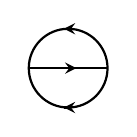
\begin{tikzpicture}[scale=0.5, baseline=-0.15cm, thick, >=stealth]
                    \draw (0, 0) circle [radius = 1cm];
                    \draw (-1, 0) -- (1, 0);
                    \draw[->] (-0.1, 1) -- ++ (-0.01, 0);
                    \draw[->] (-0.1, -1) -- ++ (-0.01, 0);
                    \draw[->] (0.2, 0) -- ++ (0.01, 0);
                \end{tikzpicture}
                \quad \text{and} \quad
                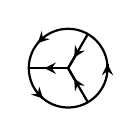
\begin{tikzpicture}[scale=0.5, baseline=-0.15cm, thick, >=stealth]
                    \draw (0, 0) circle [radius = 1cm];
                    \draw (0, 0) -- (60:1);
                    \draw (0, 0) -- (-60:1);
                    \draw (0, 0) -- (180:1);
                    \draw[-<] (0, 0) -- (60:0.6);
                    \draw[-<] (0, 0) -- (-60:0.6);
                    \draw[->] (0, 0) -- (180:0.6);
                    \draw[->] (1, 0.1) -- ++ (0, 0.01);
                    \draw[->] (140:1) -- ++ (225:0.01);
                    \draw[->] (230:1) -- ++ (-45:0.01);
                \end{tikzpicture}
            \end{equation*}
            \item These are just traces of Young projectors
        \end{itemize}
    \end{frame}
    
    \begin{frame}{How are Hermitian Young Projectors defined?}
        \begin{itemize}
            \item Let \(Y_{\Theta}\) be the Young projector corresponding to the \(n\) box Young tableau \(\Theta\)
            \item Let \(\Theta'\) be the Young tableau given by removing the \(n\)th box from \(\Theta\)
            \item Then \(P_{\Theta}\) are the Hermitian Young projectors defined recursively by
            \begin{equation*}
                P_{\Theta} = 
                \begin{cases}
                    Y_{\Theta} & n \le 2,\\
                    (P_{\Theta'} \otimes I)Y_{\Theta}(P_{\Theta'} \otimes I) & n > 2.
                \end{cases}
            \end{equation*}
        \end{itemize}
        \begin{equation*}
            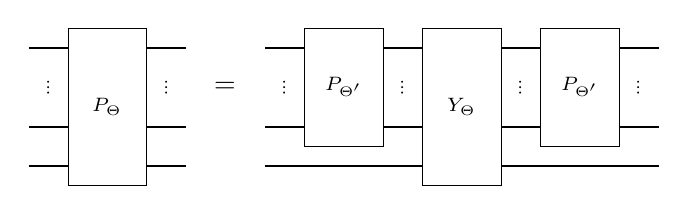
\begin{tikzpicture}[baseline=(equal.base), font=\scriptsize, wire/.style={thick}]
                \draw (0, -0.25) rectangle (1, 1.75) node [midway] (Ptheta) {\(P_{\Theta}\)};
                \draw[wire] (-0.5, 0) -- (0, 0);
                \draw[wire] (-0.5, 0.5) -- (0, 0.5);
                \draw[wire] (-0.5, 1.5) -- (0, 1.5);
                \node at (-0.25, 1) {\(\vdots\)};
                \draw[wire] (1, 0) -- (1.5, 0);
                \draw[wire] (1, 0.5) -- (1.5, 0.5);
                \draw[wire] (1, 1.5) -- (1.5, 1.5);
                \node (A) at (1.25, 1) {\(\vdots\)};
                \draw (3, 0.25) rectangle (4, 1.75) node [midway] {\(P_{\Theta'}\)};
                \draw[wire] (2.5, 0) -- (4.5, 0);
                \draw[wire] (2.5, 0.5) -- (3, 0.5);
                \draw[wire] (2.5, 1.5) -- (3, 1.5);
                \node (B) at (2.75, 1) {\(\vdots\)};
                \draw[wire] (4, 0.5) -- (4.5, 0.5);
                \draw[wire] (4, 1.5) -- (4.5, 1.5);
                \node at (4.25, 1) {\(\vdots\)};
                \draw (4.5, -0.25) rectangle (5.5, 1.75) node [midway] {\(Y_{\Theta}\)};
                \draw[wire] (5.5, 0) -- (7.5, 0);
                \draw[wire] (5.5, 0.5) -- (6, 0.5);
                \draw[wire] (5.5, 1.5) -- (6, 1.5);
                \node at (5.75, 1) {\(\vdots\)};
                \draw (6, 0.25) rectangle (7, 1.75) node [midway] {\(P_{\Theta'}\)};
                \draw[wire] (7, 0.5) -- (7.5, 0.5);
                \draw[wire] (7, 1.5) -- (7.5, 1.5);
                \node at (7.25, 1) {\(\vdots\)};
                \node (equal) at ($(A)!0.5!(B)$) {\normalsize\(=\)};
            \end{tikzpicture}
        \end{equation*}
    \end{frame}
    
    \begin{frame}{What are those other Groups}
        \(\specialUnitary(n)\) is the group of unitary transformations of \(\complex^n\) with determinant one.
        
        \(\specialOrthogonal(n)\) is the group of orthogonal transformations of \(\reals^n\) with determinant one.
        
        \(\specialOrthogonal(1, 3)\) is the group of proper Lorentz transformations in \(1 + 3\) dimensions.
        
        \(\symplectic(2n)\) is the group of transformations of \((q_1, \dotsc, q_n, p_1, \dotsc, p_n)\) preserving Hamilton's equations,
        \begin{equation*}
            \dot{q}_i = \diffp{H}{p_i}, \quad\text{and}\quad \dot{p}_i = -\diffp{H}{q_i}.
        \end{equation*}
        Alternatively, transformations of \(\quaternions^{2n}\) preserving \(\overline{x}_iy_i\) with \(x, y \in \quaternions^{2n}\) quaternion \enquote{vectors}. {\tiny Since quaternion multiplication is not commutative \(\quaternions\) is not a field, but it is a ring, so \(\quaternions^{2n}\) is an \(\quaternions\)-module, not a vector space.}
    \end{frame}
\end{document}
